\subsection{Experiment \rnum{1}: File Loading and Data Processing}

\begin{figure}[!h]
    \centering
    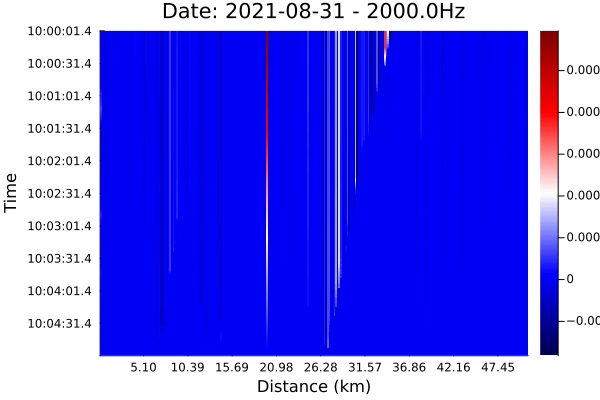
\includegraphics[width=0.8\linewidth]{figures/heatmap_das_test.png}
    \caption{Heatmap displaying 5 minutes of loaded \acrshort{das} data}
    \label{fig:dasoutput}
\end{figure}

\begin{figure}[!h]
    \centering
    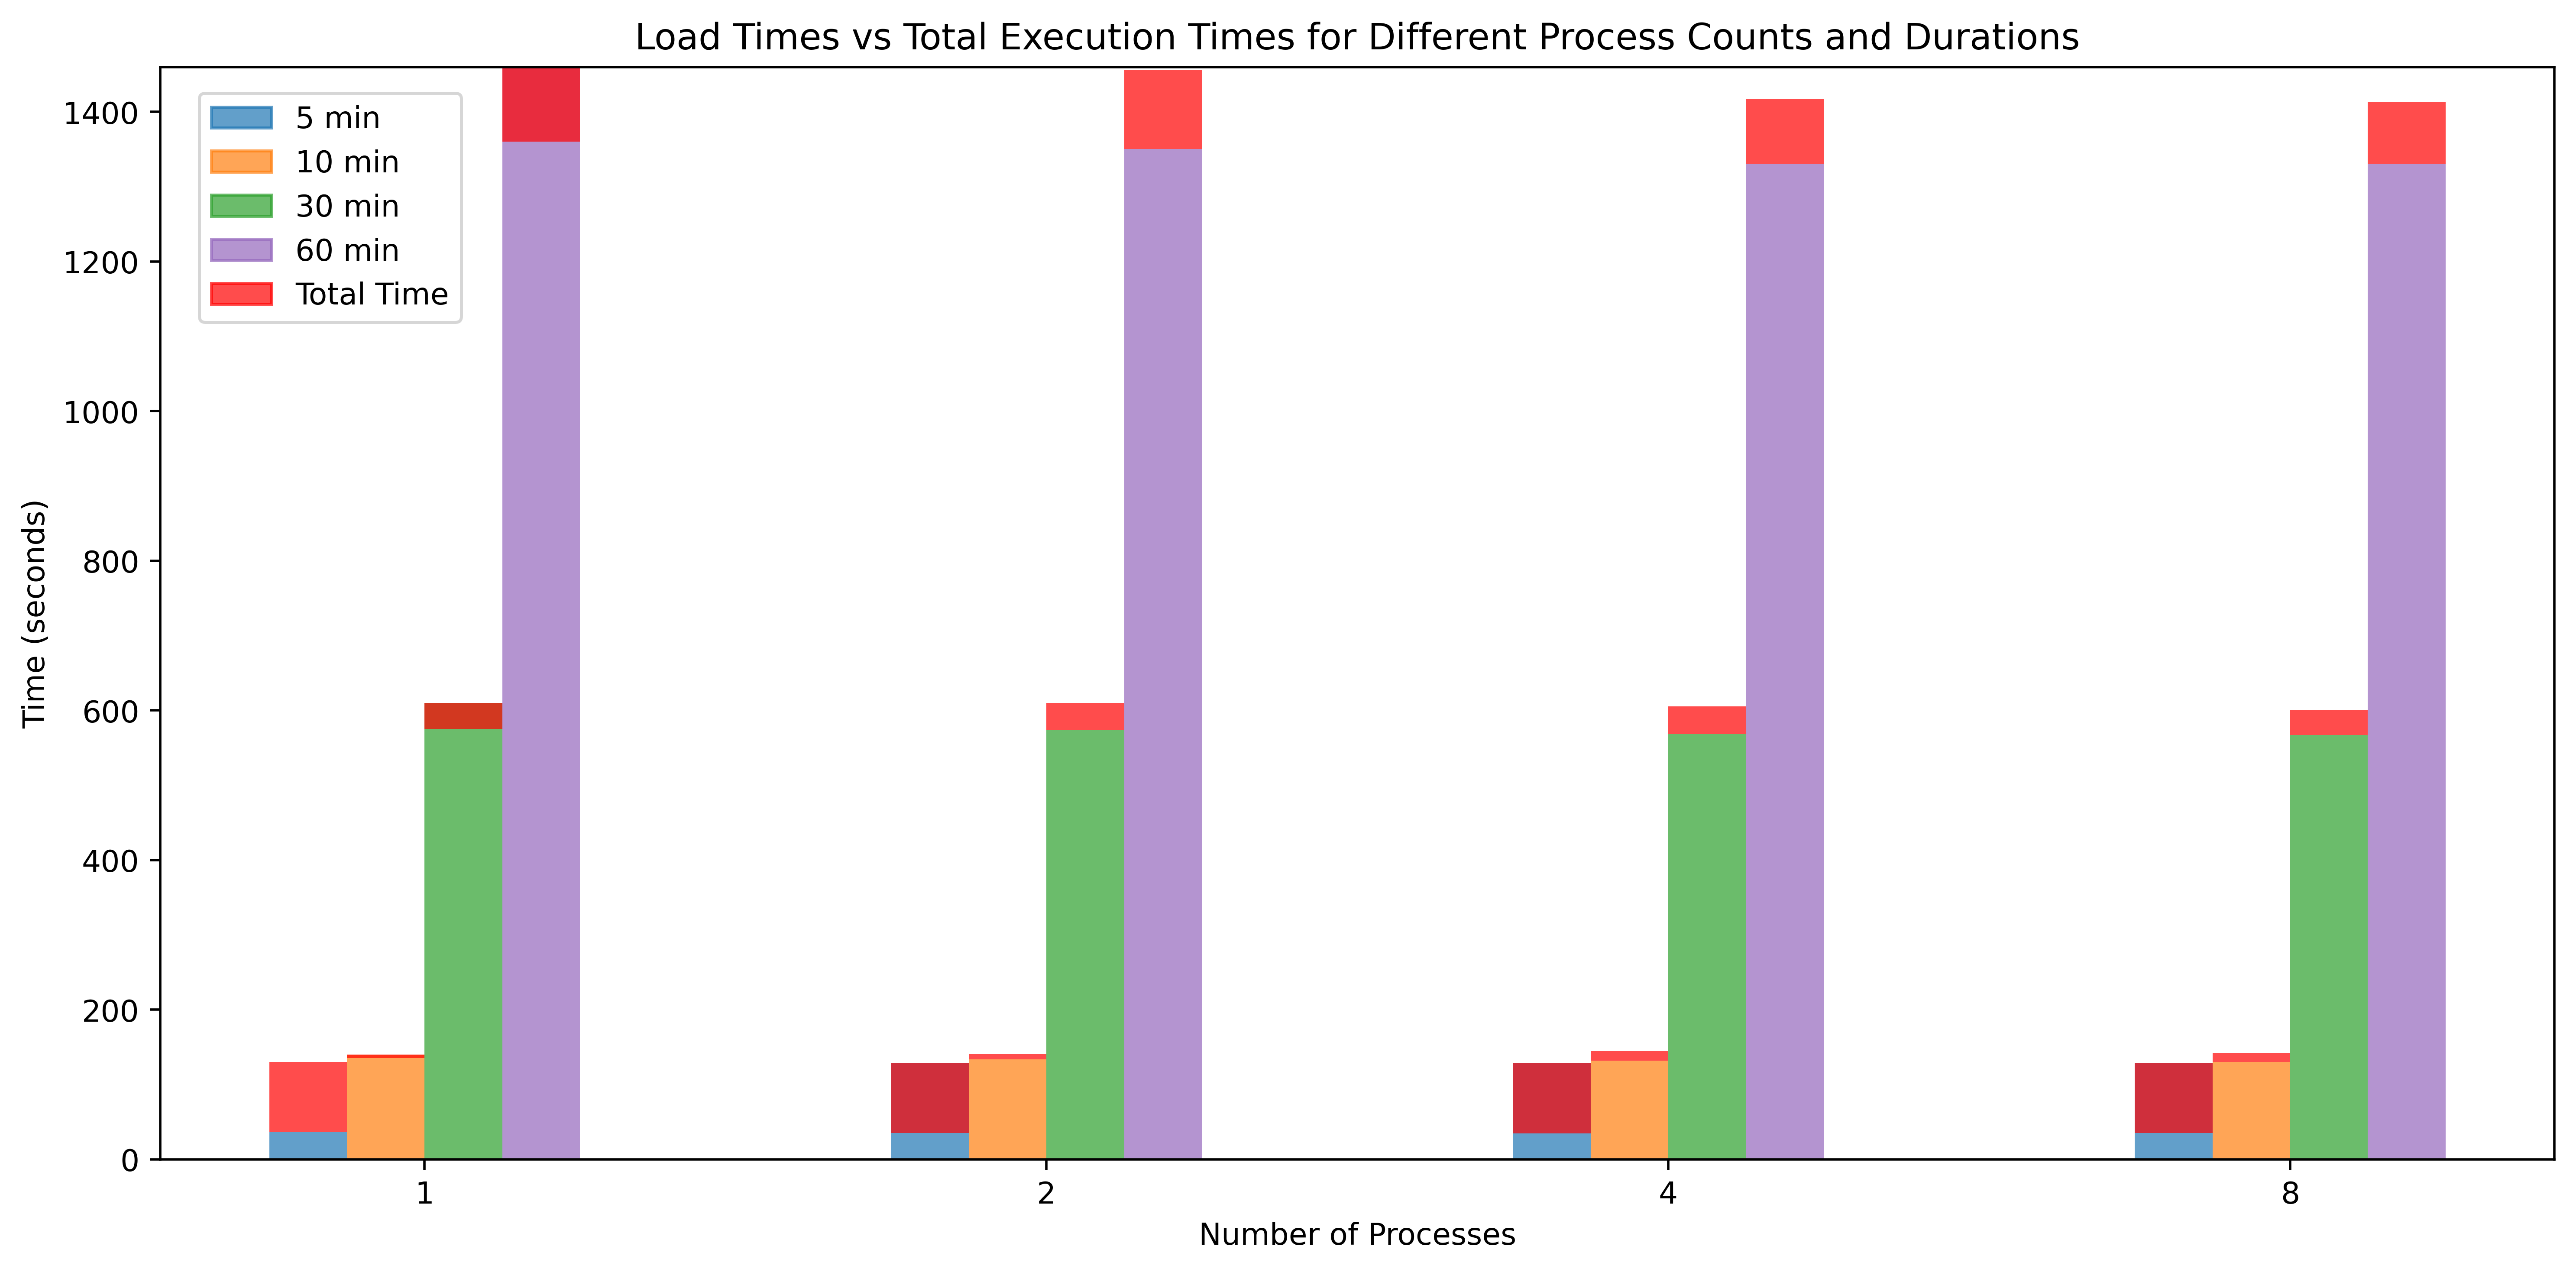
\includegraphics[scale=0.50]{figures/judasex.png}
    \caption{Loading and total processing execution times for different durations and processes. The red top indicates the total runtimes, while the other colors show the duration of the \lstinline{load_DAS_files} function for the different durations. \footnote{Claude AI was used to fix the spacing between bars}}
    \label{fig:judasextime}
\end{figure}

Figure \ref{fig:judasextime} highlights the load section's portion. This is the most resource-intensive portion of the program for all processes and file duration except the 5-minute block. 


\begin{figure}[!htbp]
\centering
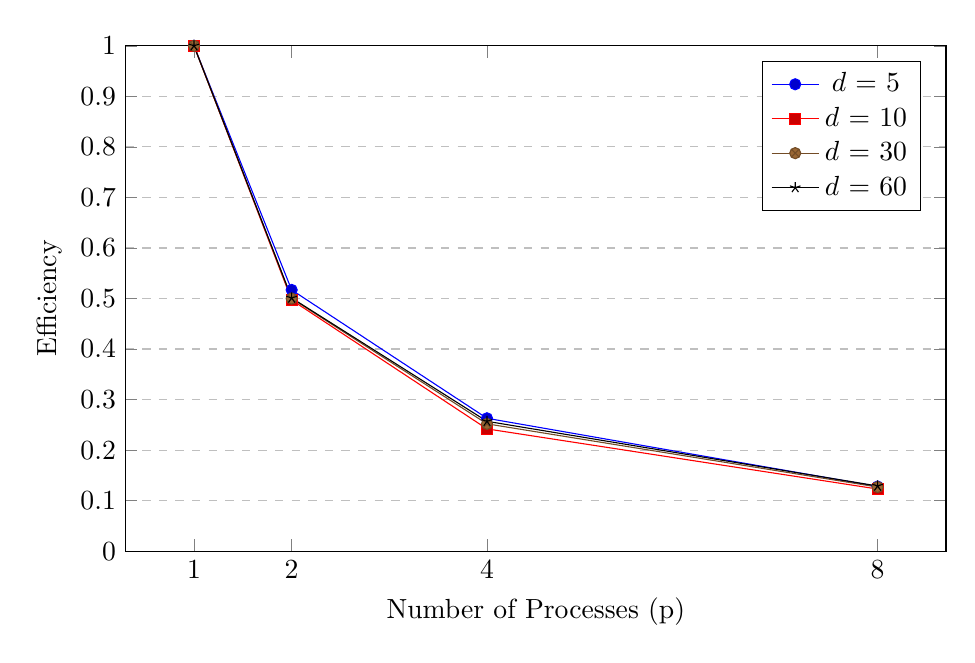
\begin{tikzpicture}
\begin{axis}[
    ylabel={Efficiency},
    xlabel={Number of Processes (p)},
    xticklabels={1,2,4,8},
    xtick={1,2,4,8},
    ytick={0.0, 0.1, 0.2, 0.3, 0.4, 0.5, 0.6, 0.7, 0.8, 0.9, 1.0},
    legend pos=north east,
    ymajorgrids=true,
    grid style=dashed,
    width=12cm,
    height=8cm,
    ymax=1,
    ymin=0,
]
\addplot coordinates {(1,1) (2,0.517) (4,0.263) (8,0.128)};
\addplot coordinates {(1,1) (2,0.497) (4,0.242) (8,0.123)};
\addplot coordinates {(1,1) (2,0.500) (4,0.252) (8,0.127)};
\addplot coordinates {(1,1) (2,0.501) (4,0.257) (8,0.129)};
\legend{$d$ = 5, $d$ = 10, $d$ = 30, $d$ = 60}
\end{axis}
\end{tikzpicture}
\caption{Efficiency for different problem sizes and process counts. $d$ is the loaded signal duration in minutes.}
\label{fig:judasefficiency}
\end{figure}
